In this section, we present our static program analysis algorithm for computing 
% an upper bound on the 
% execution-based reachability times 
the \emph{reachability-bound} for every program point $l$ in a program $c$ in a path sensitive manner.
% , as defined in last section.
%
% In order to have the upper bound of the reachability for every label of a program $c$, we design 
% a path sensitive reachability bound analysis algorithm {\THESYSTEM}.
The algorithm is summarized into the following steps,
% \begin{figure}
%   \centering    
% 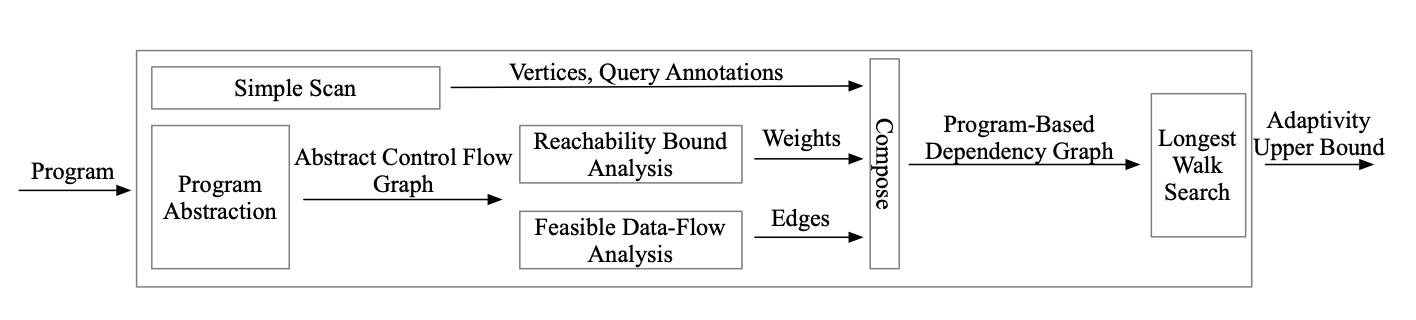
\includegraphics[width=1.0\columnwidth]{adapfun.png}
%   \vspace{-0.3cm}
%   \caption{The overview of {\THESYSTEM}}
%   \label{fig:adaptfun}
%   \vspace{-0.5cm}
% \end{figure}
%
\\
% \framebox{
    % \text{
    1. Compute Abstract Transition graph, $\absG(c)$ through program abstraction.
    % }
    \\
    % \text{
    2. Compute refined program by \cite{GulwaniJK09}. $\rprog = API(\absG(c))$
    \\
    3. Compute local bound $\outinB(\tpath, c)$
    \\
    4. Compute Reachability-Bound $\psRB = \inoutB(\tpath, c)$
    % }
% }
%
\begin{enumerate}
\item  In Section~\ref{sec:progabs}, we first construct an abstract transition graph based on $c$, by computing an abstract transition 
for every labeled command. 
This graph is used in the following sections
%  from Section~\ref{sec:refine} to Section~\ref{sec:psrbcompute} 
for computing the path-sensitive reachability-bound of a program location.
% see Section~\ref{sec:alg_vertexgen}
\item The second step in Section~\ref{sec:refine}
refines the multiple-paths loops in the program
% this program path sensitively, 
based on the abstract transition graph.
This step transforms the multiple-paths loops into multiple loops where
the interleaving of paths is explicit.
% \item Section~\ref{sec:lbcompute} computes the ranking function  
% \footnote{\textbf{ranking function} is the named used in \cite{SinnZV14}
% and \textbf{local bound} is the name used in \cite{ZulegerGSV11}, \cite{sinn2017complexity}.
% We refer to the two names as the same meaning in this paper.} for each edge in a program's abstract transition graph,
% and estimates the upper bounds on every ranking function's maximum value and every edge's execution times path-insensitively.
% path-insensitive reachability upper bound for every while loop command in $c$.
\item Section~\ref{sec:outinalg} performs the \textbf{Outside-In} algorithm and computes
the upper bound for the execution times for every path in a refined loop locally.
It first computes the ranking function  
\footnote{\textbf{ranking function} is the named used in \cite{SinnZV14}
and \textbf{local bound} is the name used in \cite{ZulegerGSV11}, \cite{sinn2017complexity}.
We refer to the two names as the same meaning in this paper.} 
for each edge in a program's abstract transition graph,
and estimates the upper bounds on every ranking function's maximum value and every path's execution times.
% , named \textbf{Outside-In} bound.
% path-sensitive local bounds.
\item Section~\ref{sec:inoutalg}
performs the \textbf{Inside-Out} algorithm and 
computes the path-sensitive reachability-bound for every program point,
It first computes the upper bound for the execution times of
every simple path in the refined program globally. 
Then it sums up the bounds of paths contains certain program point as its path-sensitive reachability-bound.
%  named \textbf{Inside-Out} bound.
% abstract transition graph.
% \item Section~\ref{sec:psrbcompute} computes the path-sensitive reachability-bound for every program point
% %  in this program 
% based on the above results.
%  by
%  ?summarizing 
% the path-sensitive reachabilitybound of each edge on the abstract transition graph.
% \item The Section~\ref{sec:reachabilitybound_algorithm} computes program's reachability bound in two steps as follows.
\end{enumerate}